\documentclass[]{softeng}

\title{Proposta di progetto Home Banking}
\date{\today}

\begin{document}

\maketitle

\section{Visione del sistema}

Si vuole realizzare un sistema di Home Banking rivolto a persone fisiche (retail banking).
Considerata la necessit\`a crescente di aumentare la trasparenza bancaria e i controlli fiscali automatizzati, il governo ha varato\footnote{Quanto segue non rispecchia interamente la realt\`a.} un pacchetto di leggi che impone alle societ\`a di credito italiane di adeguarsi allo standard OBP\footnote{Open Bank Project: \url{https://openbankproject.com/}} gi\`a in uso in Germania e nel Regno Unito\footnote{\url{http://opensource.com/business/15/4/open-standard-api-banking}}.
In questo contesto di transizione, la nostra societ\`a si propone di progettare un'applicazione che faccia da front-end per una banca che abbia adottato lo standard OBP.

Lo standard OBP \`e fondamentalmente un metodo standardizzato di accesso ai dati contenuti nel back-end della banca.
Nel momento in cui si adegua allo standard, ogni banca mantiene inalterate la struttura del suo database e dei sistemi preesistenti atti alla gestione delle operazioni bancarie.
Il software di OBP agisce quindi da \emph{wrapper} del sistema preesistente, mascherando completamente e rendendo inaccessibili le interfacce del backend, ed esponendo all'esterno unicamente le interfacce definite dallo standard.

\graphicspath{{Images/}}
\begin{figure}[tp]
	\centering
	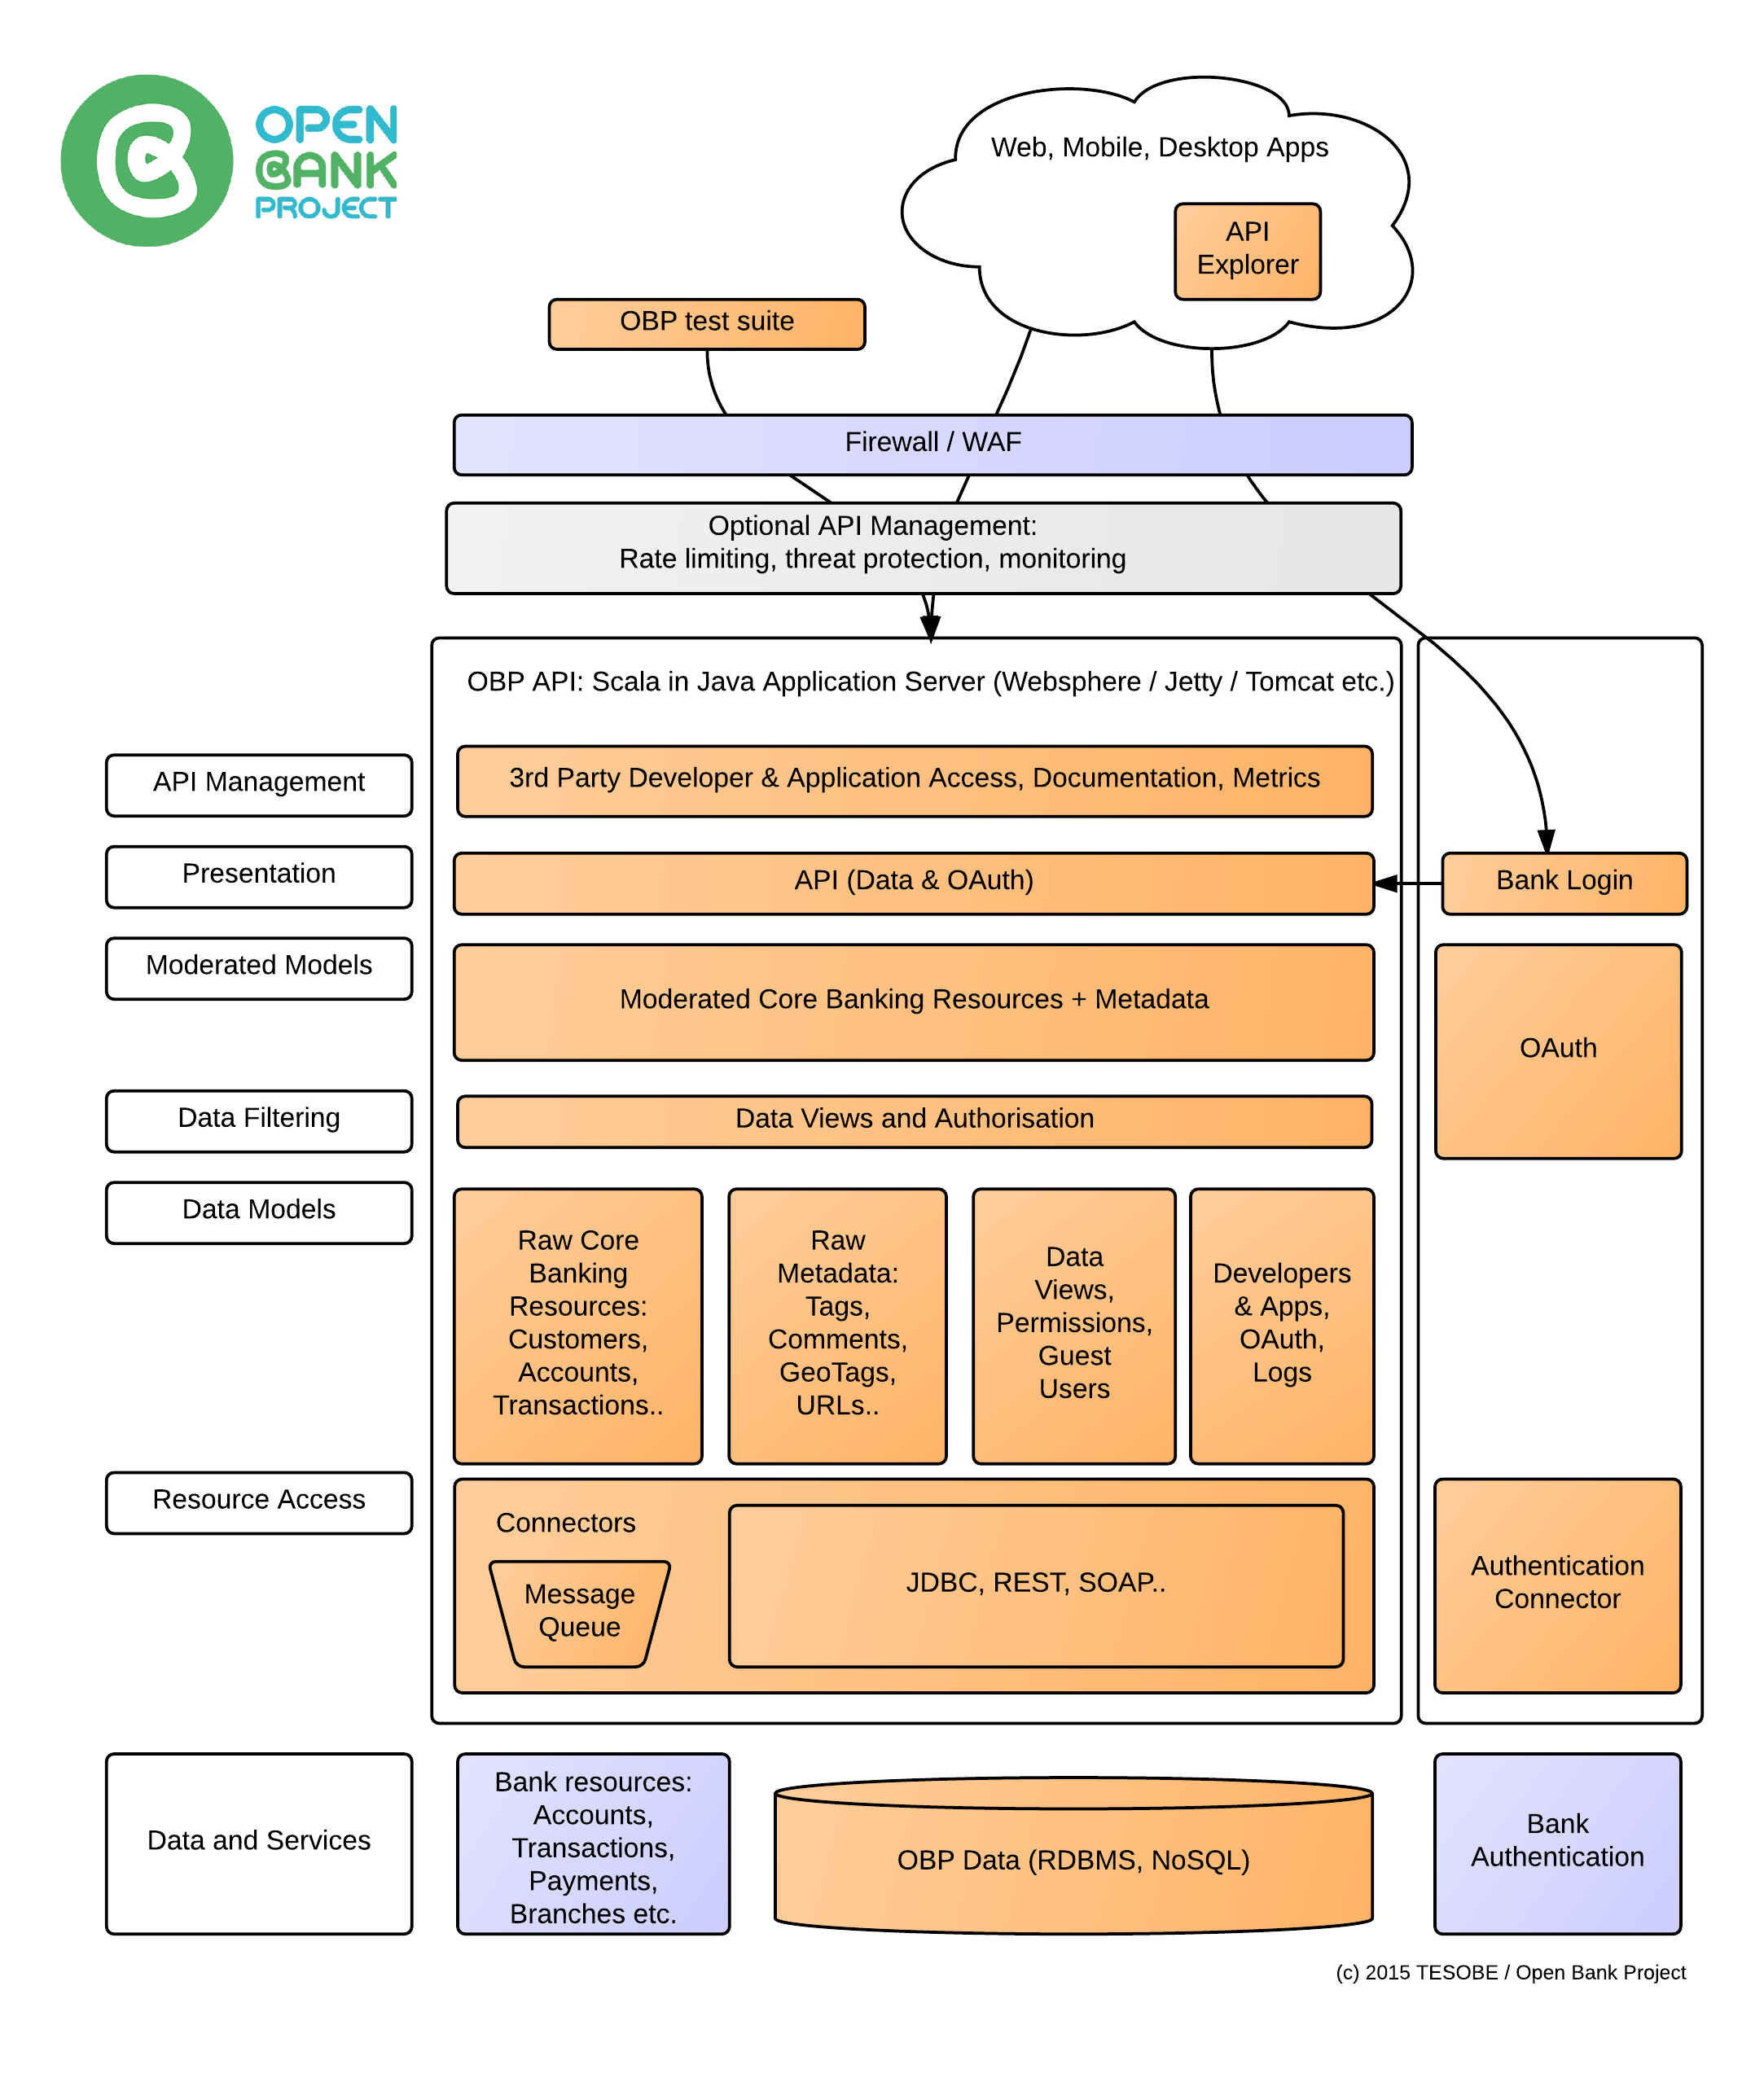
\includegraphics[width=\textwidth]{open_bank_project_architecture}
	\caption{Architettura del software di Open Bank Project. \url{https://github.com/OpenBankProject/OBP-API/wiki/Open-Bank-Project-Architecture}}
	\label{fig:open_bank_project_architecture}
\end{figure}
% TODO inserire diagramma architetturale di OBP

La nostra applicazione permetter\`a ai clienti di effettuare le normali operazioni bancarie da casa, accedendo al sito della banca tramite web browser.

Il nostro sistema dovr\`a:
\begin{enumerate}
	\item Permettere la registrazione online di nuovi clienti.
		La registrazione deve essere ultimata presso una filiale della banca.
	\item Utilizzare lo standard TOTP\footnote{CIAO}.
	\item Permettere all'utente di effettuare le seguenti operzioni:
		\begin{enumerate}
			\item visualizzare il saldo (contabile, disponibile e liquido)
			\item visualizzare lo storico delle transazioni effettuate
			\item gestire le proprie carte di credito e carte prepagate
			\item disporre pagamenti di vario tipo (bonifici ordinari, bonifici SEPA, ricariche prepagate, ricariche telefoniche, pagamenti bollettini, etc)
			\item gestire portafogli fondi, azioni, obbligazioni e titoli statali % TODO CHECK SYNTAX
		\end{enumerate}
	\item Permette di effettuare l'audit di sicurezza agli addetti della banca.
	\item Notificare all'utente (tramite SMS e/o email) determinati eventi.
\end{enumerate}

Simuleremo la realizzazione del progetto seguendo lo Unified Process, producendo la documentazione richiesta da ogni iterazione e flusso di lavoro.
L'implementazione del sistema non fa parte di questo progetto.

\section{Documentazione}

La documentazione che produrremo comprender\`a:
\begin{enumerate}
	\item Studio di fattibilit\`a e analisi del contesto.
	\item Specifica dei requisiti e modello di business.
	\item Documento di analisi dei rischi.
	\item Bozza di contratto per il cliente (basata sulla specifica dei requisiti prodotta).
	\item Analisi del sistema % TODO espandere
	\item Analisi dei costi e pianificazione temporale.
	\item Piano dei test.
\end{enumerate}
L'ordinamento dei documenti non \`e vincolante, ma \`e stato opportunamente scelto per i seguenti motivi:
\begin{itemize}
	\item L'analisi dei rischi precede la bozza di contratto perch\'e il sistema che intendiamo sviluppare ha forti requisiti di sicurezza, ed \`e opportuno iniziare l'analisi dei rischi nelle fasi iniziali del processo software.
\end{itemize}

%--------------------------------------------------------------

% TODO ripulire questa parte e spostare tutto nel file dei requisiti
Per rafforzare i requisiti non funzionali (come i requisiti di sicurezza) si sceglie di rivolgere il sistema di Home Banking a persone fisiche (retail banking).

Alcune delle funzionalit\`a che il sistema pu\`o offrire sono:
\begin{enumerate}
	\item L'utente si deve poter pre-registrare online fornendo i suoi dati anagrafici, e:
		\begin{enumerate}
			\item se l'utente ha gi\`a un conto aperto con la banca, pu\`o fornire il suo numero di conto;
			\item se l'utente non ha gi\`a un conto con la banca, pu\`o scegliere diverse soluzioni con agevolazioni differenti e pre-compilare i moduli necessari all'apertura del conto.
				% TODO: cambiare "se l'utente ha gi\`a un conto con la banca" in "se l'utente desidera aprire un nuovo conto"
		\end{enumerate}
		Un utente pre-registrato pu\`o recarsi presso una filiale della banca e ultimare la registrazione presentando il documento d'identit\`a.
		La banca gli fornir\`a le informazioni per l'accesso.
		Ai nuovi clienti viene fornito su richiesta un bancomat.
		% TODO: rimuovere, non \`e di interesse per l'applicazione, facciamo home banking non ATM

		Un utente non pre-registrato pu\`o effettuare la procedura completa di registrazione presso una filiale, fornendo le stesse informazioni richieste agli utenti che si pre-registrano online.
	\item Le informazioni per l'accesso comprendono:
		\begin{enumerate}
			\item Il numero di conto;
			\item La password del conto;
			\item Un dispositivo TOTP\footnote{Time-Based One Time Password, RFC 6238. \url{https://tools.ietf.org/html/rfc6238}} per effettuare operazioni sensibili.
		\end{enumerate}
	\item Un utente registrato pu\`o effettuare il login al sistema di Home Banking fornendo le informazioni di accesso (requisito TOT), in particolare deve inserire numero di conto e password del conto.
	\item Un utente che ha effettuato l'accesso al sistema di Home Banking deve poter svolgere le seguenti operazioni senza fornire la One Time Password:
		\begin{enumerate}
			\item Visionare saldo contabile, disponibile e liquido.
			\item Visionare uno storico delle transazioni effettuate.
			\item Visionare informazioni riguardo le carte di credito collegate al conto (se presenti).
			\item Effettuare ``operazioni veloci'' impostate attraverso un sistema di configurazione (requisito TOT).
		\end{enumerate}
	\item Un utente che ha effettuato l'accesso al sistema di Home Banking deve poter effettuare le seguenti operazioni fornendo ogni volta la One Time Password:
		\begin{enumerate}
			\item Effettuare transazioni, come:
				\begin{enumerate}
					\item bonifici ordinari e bonifici SEPA;
					\item ricariche carte prepatate e schede telefoniche;
					\item pagamento bollette, bollettini, tasse, etc;
				\end{enumerate}
			\item Configurare operazioni veloci.
			\item Se ci viene in mente altro ce lo mettiamo.
		\end{enumerate}
	\item Ogni operazione deve essere registrata in un log.
		Devono essere mantenute le seguenti informazioni:
		\begin{enumerate}
			\item l'operazione eseguita;
			\item il conto coinvolto nell'operazione;
				% TODO rivedere codesta parte: codice univoco della transazione al posto del conto?
				% analizzare bene come funziona OBP
			\item l'istante dell'operazione;
			\item informazioni riguardanti il terminale da cui \`e stata effettuata l'operazione.
		\end{enumerate}
	\item Il sistema deve poter essere configurabile dall'utente per inviare notifiche via SMS e/o via email a seguito di ogni evento stabilito dall'utente.
		La banca pu\`o associare una tariffa per abilitare le notifiche su specifici insiemi di eventi.
		Gli eventi notificabili possono includere:
		\begin{enumerate}
			\item Accesso al sistema;
			\item Pagamento o prelievo dal conto;
			\item Pagamento ricevuto.
		\end{enumerate}
\end{enumerate}

\end{document}

